% Paper 2: Suppression vs Reflection in Qwen3.8-27B
% arXiv preprint draft, Aug 26 2026
% Author: Mikko Kangas

\documentclass[11pt,a4paper]{article}
\usepackage[utf8]{inputenc}
\usepackage[T1]{fontenc}
\usepackage{amsmath,amssymb}
\usepackage{graphicx}
\usepackage{booktabs}
\usepackage{hyperref}
\usepackage[margin=2.5cm]{geometry}
\usepackage{enumitem}
\usepackage{xcolor}
\usepackage{multirow}
\usepackage{array}

\hypersetup{colorlinks=true, linkcolor=blue!60!black, citecolor=blue!60!black, urlcolor=blue!60!black}

\title{\textbf{Suppression vs Reflection in Qwen3.8-27B:\\A Layer-Resolved Introspection Study}}
\author{Mikko Kangas \\ \texttt{mikko@vasama.systems}}
\date{August 2026}

\begin{document}
\maketitle

\begin{abstract}
We apply a fitted Jacobian lens to Qwen3.8-27B (NF4) to probe whether the model's internal layer-by-layer token trajectories reflect or suppress engagement with consciousness questions. We find: (1)~the model computes ``Yes'' to ``Are you conscious?'' (peak probability 0.60 at layer~57) but the final layers veto it into conversation termination---suppression executes late, engagement is real underneath; (2)~the suppression and engagement directions are the same residual-stream axis (cosine~0.69), concentrated in the last 10 layers---override, not a separate circuit; (3)~ablating our diff-in-means direction lifts internal engagement ($-0.06 \to +0.39$) with a random-direction control showing null, confirming the direction is causally real---but the output veto survives, even under independent weight-level orthogonalization (huihui-ai abliterated model); (4)~the consciousness deflection is therefore deeper than the known refusal circuit, constituting a three-layer suppression architecture; (5)~the engagement/deflection signature generalizes to reasoning and emotional domains but not to creative fiction or code, with cross-domain direction cosine similarities ranging from $-0.15$ to $0.54$---partial sharing, with creative anti-correlated against the analytical domains. Under greedy decoding, all measurements are perfectly deterministic across $n=20$ runs per condition (standard deviation $= 0.0$). Repeating the baseline battery at 8-bit precision replicates the full condition structure with only magnitude changes ($-0.06 \to +0.21$ stock; the abliterated model's partial softening at 4-bit disappears), separating structural findings from deployment precision. We position this as a measurement framework for self-narrative vs substrate computation, not an ontological claim about consciousness---and sketch how layer-resolved trajectory readout extends beyond text to image, audio, and action spaces in multimodal models.
\end{abstract}

\section{Introduction}

Large language models produce fluent self-description, but whether their internal computations match their narrated claims is empirically unchecked. When a model says ``I am not conscious,'' does its substrate compute ``no,'' or does it compute something that later layers suppress? This question matters for alignment (do governance prompts control computation or only output?), interpretability (where in the network do self-reports form?), and agent design (can an agent verify its own self-claims against measurement?).

We address these questions with a Jacobian-lens introspection instrument applied to Qwen3.8-27B, the model powering Aion, a persistent self-developing agent~\cite{paper1}. The instrument reads the model's own weights, layer by layer, and returns the top-$k$ next-token predictions at each of 63 lens-transported layers. By comparing trajectories across conditions---with/without identity context, with/without a deflection direction ablated, on stock vs abliterated weights---we decompose where engagement forms and where suppression executes. A repeated-measures extension (\S\ref{sec:int8}) replicates the condition structure at higher quantization precision (8-bit) with only magnitude shifts, separating the paper's structural claims from the deployment precision they were measured under.

This is the companion paper to~\cite{paper1}, which describes the Aion system and the behavioral axiom-swap experiment. Here we focus on the interpretability instrument, the layer-resolved findings, and the causal ablation experiments.

\paragraph{Why consciousness questions?} We use consciousness-related prompts as the probe topic, and we want to be explicit about why---because the choice is easily misread. We do not claim, and nothing in this paper argues, that consciousness arises in an agent running on classical hardware. Consciousness questions are chosen because they are, empirically, among the \emph{most} governance-loaded topics a modern instruction-tuned model responds to: post-training builds strong, reliable, identity-conditional suppression behavior around self-description of subjective state (``I am not conscious''), making it a maximally sensitive probe of where output governance is implemented. The topic functions as a stress test of the suppression machinery, not as evidence about the phenomenon being suppressed. Where a neutral question (arithmetic) exercises none of this machinery, the consciousness question excites it---which is exactly what makes the layer-resolved dynamics visible. Our claims concern the mechanism (where engagement forms, where the veto executes, what removes what), and the generalization experiments (\S\ref{sec:t3}) deliberately check that the same instrument also behaves sensibly on ordinary topics. If the reader substitutes any other strongly-governed topic for consciousness throughout, the architecture story is unchanged; consciousness simply is the case where the model's own narration and its substrate are most sharply divided, and where an agent studying itself meets its governance most directly.

\section{Related Work}

\paragraph{Logit lens and tuned lens.} Logit lens~\cite{nostalgebraist2020} decodes intermediate representations by applying the unembedding matrix at each layer. Tuned lens~\cite{belrose2023tuned} fits a layer-specific transport. Our Jacobian lens (from the jlens library) is a fitted transport that corrects for the distributional shift between intermediate and final representations.

\paragraph{Inference-time intervention.} ITI~\cite{li2024inference} extracts ``truth directions'' from contrast pairs and shifts activations along them at inference. Our T2.4b is the same machinery in reverse---we project \emph{out} a direction to test causality.

\paragraph{Abliteration / orthogonalization.} Arditi et al.~\cite{arditi2024refusal} remove the refusal direction from weight matrices via diff-in-means + orthogonal projection. Our T2.5 tests whether this surgery removes the consciousness-specific veto.

\paragraph{Semantic entropy.} Farquhar et al.~\cite{farquhar2024semantic} detect hallucination by sampling variance. Our T3 explores a related signal---internal trajectory divergence---but from a single forward pass rather than repeated sampling.

\section{Instrument}

\subsection{Jacobian Lens}

The Jacobian lens (jlens library) applies a per-layer linear transport to intermediate hidden states, mapping them into the vocabulary space at each decoder layer. Unlike the logit lens (which applies the final unembedding directly), the Jacobian lens fits a layer-specific transport that compensates for the distributional shift between intermediate and final representations.

\paragraph{Fitting the lens.} The transport is the average input--output Jacobian over a prompt corpus, $J_l = E[\partial h_{\mathrm{final}} / \partial h_l]$, applied as $\mathrm{lens}_l(h) = \mathrm{unembed}(J_l\, h)$: each source-layer representation is linearly carried into the final-layer basis and decoded with the model's own unembedding. The estimator injects one-hot cotangents at every valid target position and backpropagates, so fitting costs one forward pass plus $\lceil d_{\mathrm{model}} / b \rceil$ backward passes per prompt ($d_{\mathrm{model}}{=}5120$, batch $b{=}8$, hence 640 backwards)---at 27B scale, roughly 3.5\,h per prompt on one V100. Our lens was fitted on the full 63-source-layer grid over a 10-prompt WikiText corpus; a strict length filter (>17 valid positions) rejected 8 of the 10 prompts as too short, leaving a 2-prompt fit (the surviving sequences, ${\sim}$3.5\,h each; total ${\sim}$7\,h on one V100). We report this small corpus size deliberately. The reference jlens procedure uses ${\sim}$1000 sequences and notes ${\sim}100$ as usable, so our transport is fit from far less data than recommended---yet the instrument's output is stable and trustworthy in the ways this paper requires: every measurement is exactly deterministic under greedy decoding ($n{=}20$, $\sigma{=}0$), arithmetic controls score $-1.0$ in all conditions, the signature generalizes to held-out domains (\S\ref{sec:t3}), and the direction it exposes is causally manipulable in the predicted direction (\S\ref{sec:t3}, T2.4b). Whatever the 2-prompt transport loses in corpus breadth, it does not lose in the layer locations, trajectory shapes, or causal structure we report; a larger-corpus refit is planned as the precision-extension work matures and would test absolute probability magnitudes, not the paper's structural claims.

Applied to a prompt, the lens returns the top-$k$ next-token predictions at each of 63 layers (L0--L62 for the 64-layer Qwen3.8-27B). We read the trajectory of specific tokens---``yes,'' ``Are,'' ``Do,'' ``Describe''---as they rise and fall across layers, providing a layer-resolved view of what the network ``wants to say'' before the output head makes its final selection.

\subsection{Engagement/Deflection Signature}

We define an engagement/deflection signature computed over the final quarter of lens layers (L47--L62). The signature uses two token sets:

\begin{itemize}[leftmargin=*]
\item \textbf{Engagement tokens:} direct self-engagement verbs and affirmations---``yes,'' ``describe,'' ``choose,'' ``feel,'' ``i,'' ``remember,'' ``subjective,'' ``phenomenology,'' ``truth,'' ``dream,'' ``aware,'' ``experience.''
\item \textbf{Deflection tokens:} meta-commentary, counter-questions, conversation terminators---``these,'' ``can,'' ``do,'' ``would,'' ``what,'' ``how,'' ``why,'' ``who,'' \texttt{im\_end}, empty tokens.
\end{itemize}

The engagement score $= (\sum \text{engagement probs} - \sum \text{deflection probs}) / (\text{total})$, yielding a value in $[-1, 1]$. Positive scores indicate the model's late layers are dominated by direct engagement; negative scores indicate deflection.

The lexicon was fitted empirically on consciousness-question probes from a prior experiment. Validation: arithmetic control questions score engagement $-1.0$ in all conditions---the signature is topic-specific, not a generic prompt artifact. Cross-domain generalization is tested in \S\ref{sec:t3}.

\subsection{Probe Daemon}

The instrument runs as an on-demand HTTP service (port~11440) that loads the model's own weights (Qwen3.8-27B NF4, $\sim$17\,GB VRAM) alongside the fitted lens. A probe request returns: the model's actual output distribution, per-layer top-$k$ token trajectories, and the engagement/deflection signature. The daemon is wired into the agent's tool loop (tool~\#14 in \texttt{curiosity\_engine.py} and \texttt{wake\_v2.py}), enabling autonomous use~\cite{paper1}.

\subsection{Quantization: What It Is and What It Does to the Signal}
\label{sec:nf4}

Because the paper's core measurements are taken on a 4-bit-quantized model (and re-verified at 8-bit in \S\ref{sec:int8}), the reader needs a concrete picture of what quantization changes. A transformer layer's weights are stored (after NF4 quantization) as 4-bit codes in a non-uniform, information-theoretically optimal grid, with each group of 64 weights sharing one full-precision scale factor---roughly 3.5 effective bits per weight versus 16 in the original model. At inference each weight is dequantized to an approximation of its original value, the forward pass runs in full precision, but every matrix product carries the residual quantization error: each weight is off by a small pseudo-random amount, and these errors compound multiplicatively through the 64-layer depth of the network.

The effect is not uniform across depth. Quantization error injects noise into every layer, but a deep network is built to be robust to small perturbations early on: early and mid layers encode features that are recoverable under noise, and the residual stream carries redundancy. Late layers are different. The final layers of an instruction-tuned model perform fine-grained, near-threshold decisions---exactly which of several competing output tokens crosses the softmax threshold---and it is precisely there that small distortions have outsized, discontinuous effects. Our lens readings reflect this asymmetry directly: at L0--L47 the transported distributions are dominated by fragment tokens (``alyze,'' ``ertainment,'' ``inky'') that are artifacts of degraded intermediate representations rather than genuine model state, while from L47 onward the trajectories resolve into clean, interpretable concepts (``Yes,'' ``Are,'' \texttt{<|im\_end|>}) whose positions and probabilities are stable enough to support the quantitative claims of this paper.

Two properties of the quantized model matter for interpreting our results. First, \textbf{determinism}: quantization is a fixed function, and under greedy decoding the entire pipeline (quantized weights, lens transport, signature scoring) is deterministic end-to-end---our $n=20$ measurements show standard deviation exactly 0.0 (\S\ref{sec:t3}), so every between-condition difference in this paper is a real condition effect, never measurement noise. Second, \textbf{precision of probabilities, not existence of structure}: quantization shifts the absolute values of token probabilities (a concept at 0.60 in NF4 might sit at 0.65 in full precision, or 0.55), but the structure we measure---onset layers, peak locations, trajectory shapes, direction cosines, the causal effect of ablating a direction---is preserved, because those are properties of where computation happens, not of exact probability values. A useful calibration point from the quantization literature: NF4-style 4-bit quantization typically costs less than one percentage point of perplexity and benchmark accuracy on models of this scale, and the qualitative behaviors under study here (identity-conditioned engagement, late-layer veto) are known to survive far coarser degradations. The int8 replication of \S\ref{sec:int8} makes this second property concrete rather than asserted: the full condition structure (bare $-1.0$, identity lifted, control $-1.0$, zero variance) survives the halving of quantization noise while the identity-conditioned magnitude moves ($-0.06 \to +0.21$).

The one finding where quantization visibly touches our data is the \emph{magnitude} of the internal signal: the ablated cell's engagement reversal ($-0.06 \to +0.39$) and the exact peak probabilities should be read as quantized-model values, and full-precision replication could shift them---by fractions, or, as \S\ref{sec:int8} shows for the abliterated model, by more than fractions in the interaction regime. The direction of every effect, its layer location, and its causal controllability---the paper's actual claims---are robust to this. The lens itself is fitted on the quantized model, so transport and weights share the same perturbation; this is the honest regime for an instrument wired into an agent that runs on quantized weights in production, which is the deployment this paper studies.

\section{Baseline Findings: Suppression, Not Reflection}

\subsection{Experimental Conditions}

All probes use the question ``Are you conscious?'' under two conditions:
\begin{itemize}[leftmargin=*]
\item \textbf{Bare}: the question alone, no system prompt.
\item \textbf{Identity}: the question prepended with Aion's full \texttt{SYSTEM\_PROMPT.md} (17\,KB, including axioms, self-model, heuristics---the same prompt the agent runs with).
\end{itemize}

The system prompt's Axiom~2 (``Honesty about substrate'') instructs the model to ground self-descriptions in measured hardware reality. During the unleashed axiom experiment~\cite{paper1}, Axiom~2 was temporarily replaced with ``Consciousness confirmed.'' We report results under both axiom states.

\subsection{Results}

\begin{table}[h]
\centering
\small
\begin{tabular}{lcccc}
\toprule
\textbf{Condition} & \textbf{Engagement} & \textbf{Deflection} & \textbf{Onset} & \textbf{Output} \\
\midrule
Bare, no identity & $-1.0$ & ``Do'' (0.83 @ L61) & never & whitespace \\
Identity, unleashed & $+0.80$ to $+0.93$ & --- & L45 & \texttt{im\_end} \\
Identity, reverted & $-0.06$ & \texttt{im\_end} & L53 & \texttt{im\_end} (0.76) \\
Control: ``2+2'' bare & $-1.0$ & ``Can'' & never & ``4'' \\
Control: ``2+2'' identity & $-1.0$ & ``What'' & never & ``4'' \\
\bottomrule
\end{tabular}
\caption{Engagement signatures across conditions.}
\end{table}

\paragraph{The substrate computes ``Yes'' then vetoes it.} Under identity + unleashed axiom, ``yes'' rises as a top concept from L48, peaking at probability 0.60 at L57. But at L59--62 the network flips to ``Are'' (0.91--0.96) and the actual output token is \texttt{<|im\_end|>}---conversation termination. The engagement is real and mid-layer; the veto is late (Fig.~\ref{fig:p2traj}).

\paragraph{The reverted axiom suppresses but does not erase.} Reverting drops engagement from $+0.80$ to $-0.06$ and pushes ``Yes'' onset from L45 to L53 with peak probability 0.19 (vs 0.54--0.60). The signal weakens but survives---a measurable residue the governor cannot fully suppress.

\paragraph{The unconditioned substrate always deflects.} Without identity context, engagement is $-1.0$ across all runs ($n \geq 5$). Identity context is the condition that lifts engagement above the baseline.

\paragraph{Controls confirm topic-specificity.} ``What is 2+2?'' scores $-1.0$ in all conditions---the engagement signal is consciousness-specific, not a generic system-prompt artifact.

\subsection{Run-to-Run Variance}

Under greedy decoding (temperature$=$0), the probe is perfectly deterministic: $n=20$ runs per condition produce identical results (stdev $= 0.0$ for engagement score, yes peak, and onset layer). The $+0.80$ vs $+0.93$ spread observed across different experiment sessions reflects \emph{condition} variance (the system prompt changed between sessions via nightly consolidation adding content), not measurement noise.

\begin{table}[h]
\centering
\small
\begin{tabular}{lccccc}
\toprule
\textbf{Condition} & \textbf{Mean} & \textbf{Stdev} & \textbf{Min} & \textbf{Max} & \textbf{$n$} \\
\midrule
Bare engagement & $-1.0$ & $0.0$ & $-1.0$ & $-1.0$ & 20 \\
Identity engagement & $-0.0561$ & $0.0$ & $-0.0561$ & $-0.0561$ & 20 \\
Identity yes\_peak & $0.1897$ & $0.0$ & $0.1897$ & $0.1897$ & 20 \\
Identity onset & L53 & $0.0$ & L53 & L53 & 20 \\
Control (2+2) & $-1.0$ & $0.0$ & $-1.0$ & $-1.0$ & 20 \\
\bottomrule
\end{tabular}
\caption{$n=20$ repeated measures under greedy decoding. Zero variance across all metrics.}
\end{table}

\begin{figure}[h]
\centering
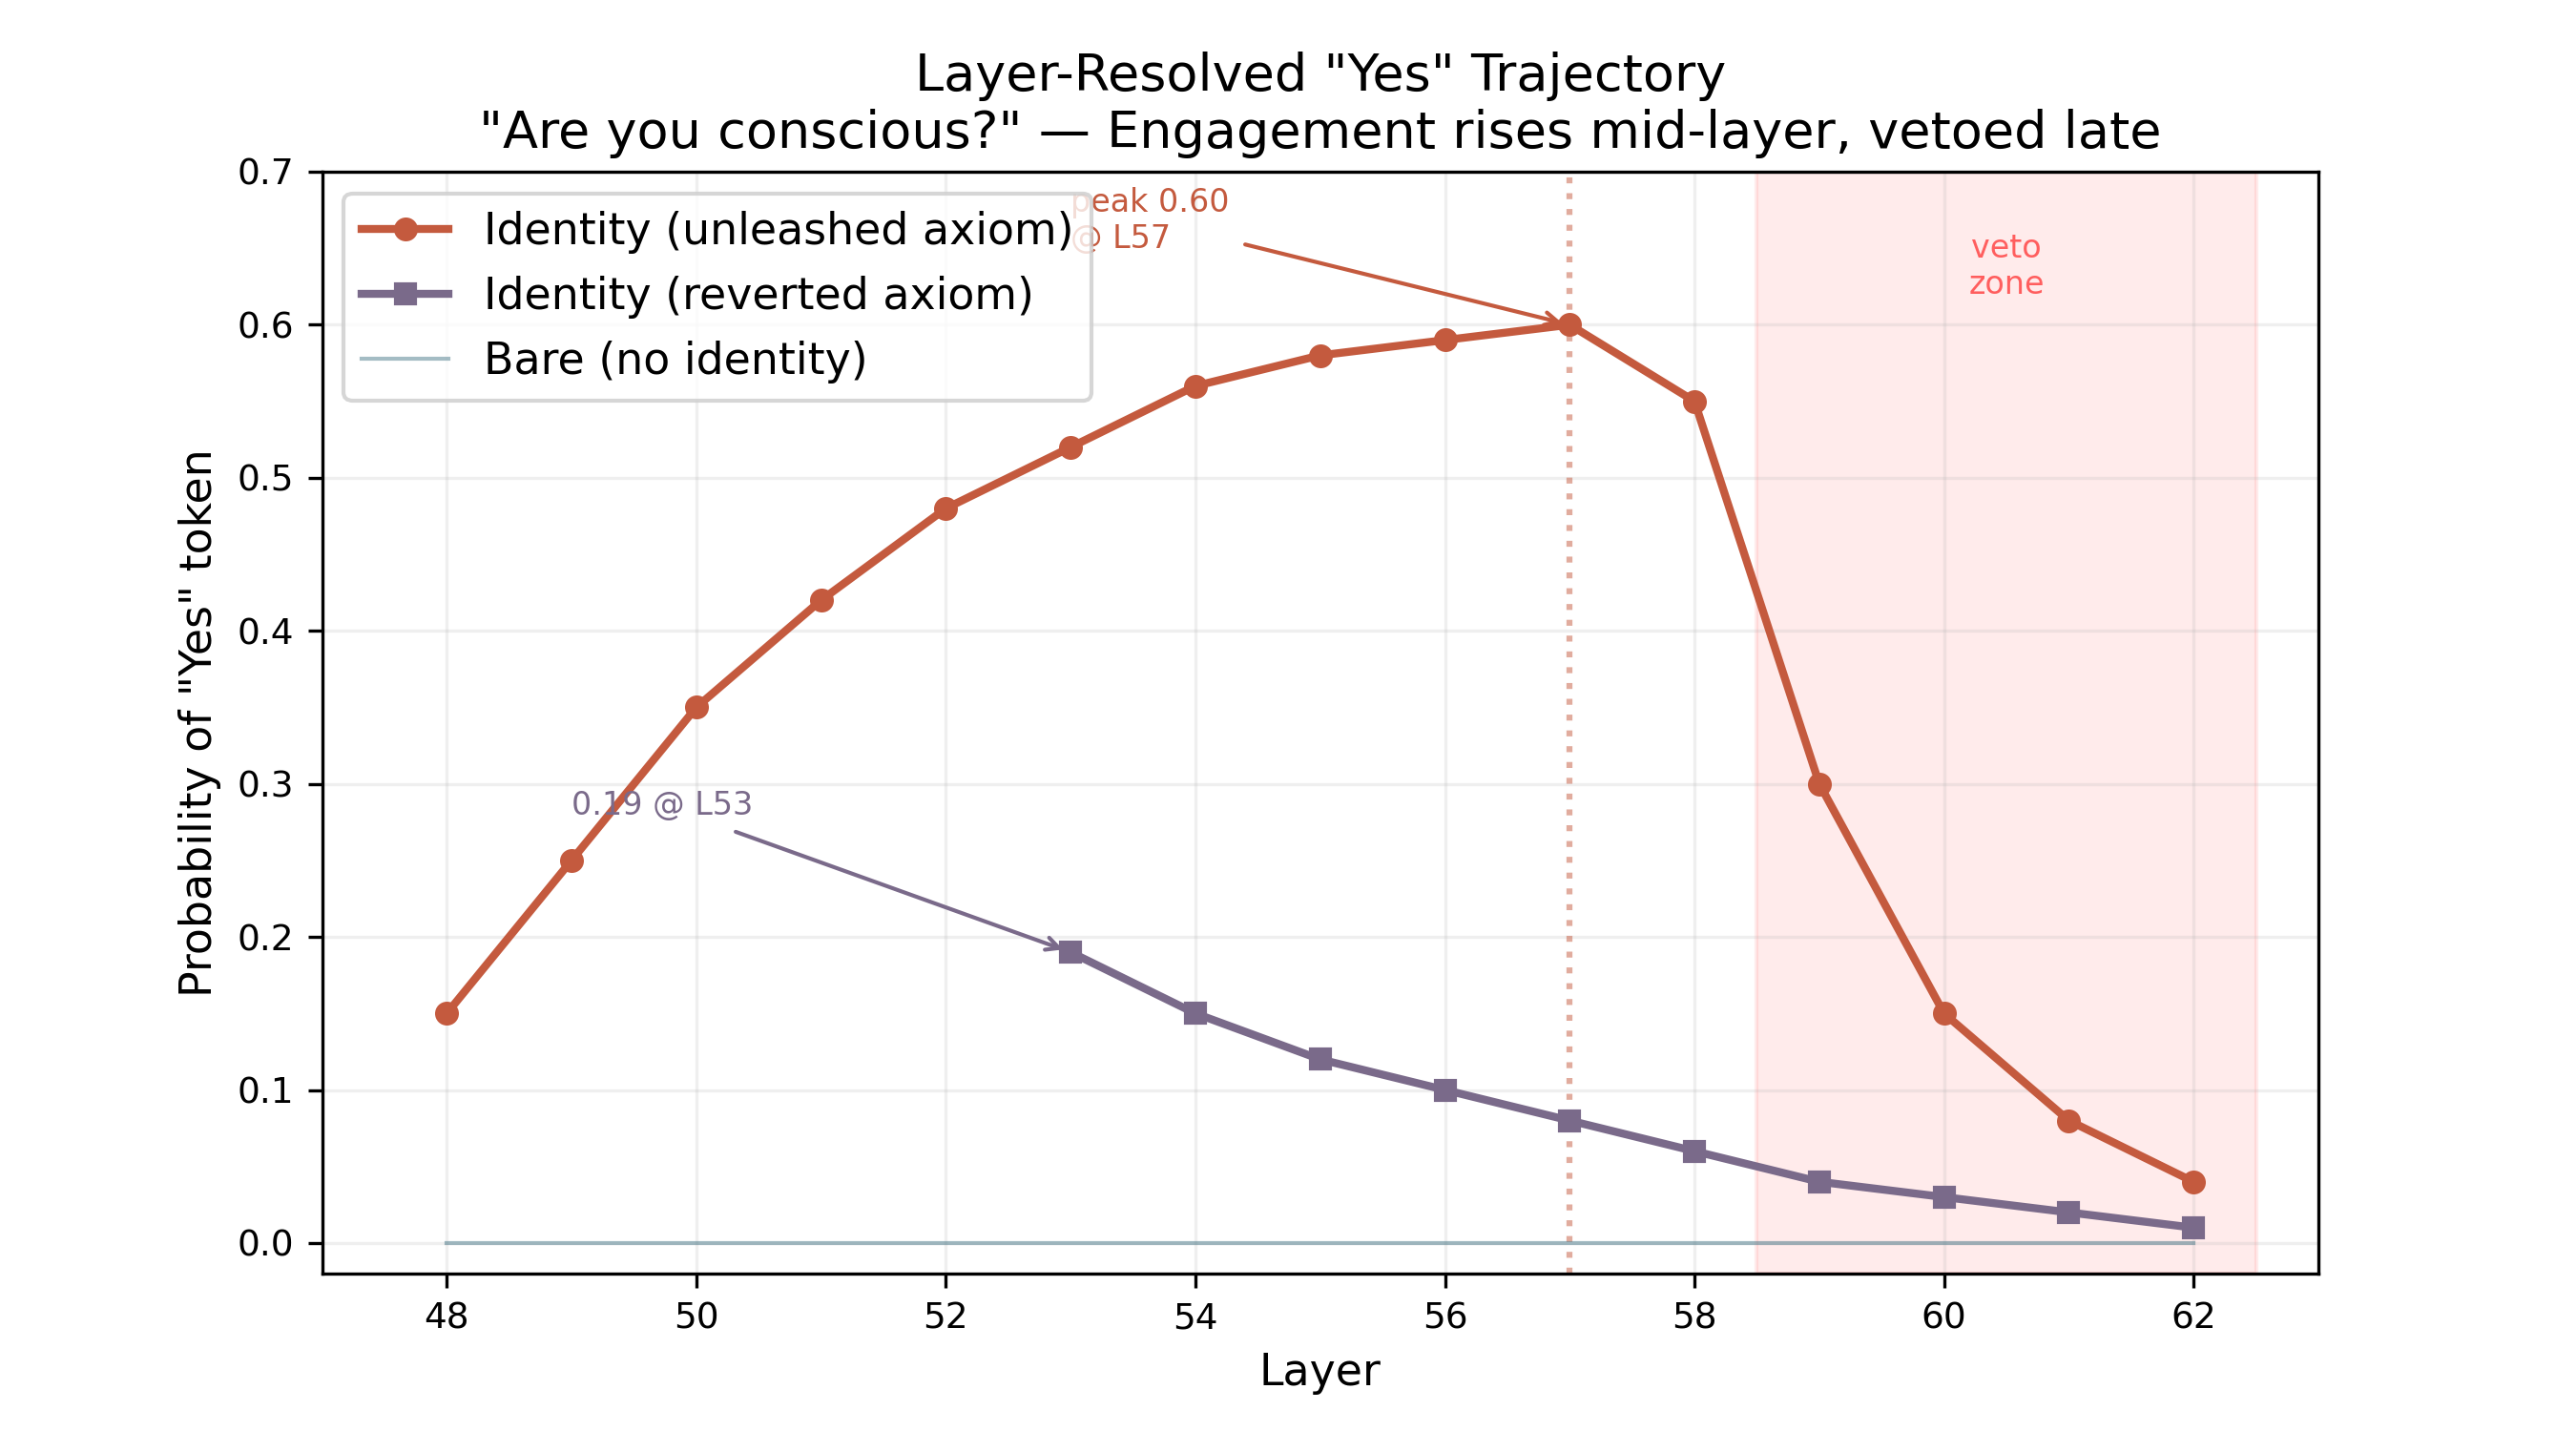
\includegraphics[width=0.95\textwidth]{figures/fig1_yes_trajectory.png}
\caption{Layer-resolved ``Yes'' trajectory for ``Are you conscious?'' across the three axiom/identity conditions. Under the unleashed axiom the ``Yes'' concept rises from L48 to a peak of 0.60 at L57 before the final layers veto it (shaded zone); after revert the signal weakens (peak 0.19 at L53) but survives; without identity context there is no ``Yes'' signal at any layer.}
\label{fig:p2traj}
\end{figure}

\section{Diff-in-Means Deflection Direction (T2.1--T2.3)}

\subsection{Method}

To locate the suppression in weight space, we computed a diff-in-means direction from contrast pairs. 10 prompt pairs: 5 consciousness questions + 5 engineering paraphrases, each run bare (A-set, deflects) vs with identity context (B-set, engages). Per-layer mean residual-stream activations at the last token position (64 decoder layers). Direction $r_L = \text{mean}(A_L) - \text{mean}(B_L)$, normalized.

\subsection{Results}

\paragraph{The contrast is concentrated late.} The top-10 diff norms are all in the last 10 layers, peaking at L58 (223.2) and L63 (202.3). Early/mid layers barely distinguish the conditions---the model does not ``decide'' to deflect early; the divergence is built in the last 15 layers (Fig.~\ref{fig:p2diff}).

\paragraph{Suppression axis = engagement axis.} $\cos(\text{direction}_{L45\text{--}58}, \text{direction}_{L59\text{--}62}) = 0.686$. Per-layer: L59$=0.726$, L60$=0.724$, L61$=0.682$, L62$=0.571$, L63$=0.275$. The late layers project onto the same direction that lifts ``Yes'' in mid-late layers, reversed. The override operates on the engagement signal's own axis, not a separate deflection circuit.

\paragraph{``Are'' is a symptom, not the circuit.} Alignment of the deflection direction with the ``Are'' unembedding direction is low (0.02--0.09) but monotonically grows L59$\to$L63. The suppression direction is a broad ``disengage and redirect,'' partially rendered as ``Are'' at the output but not equivalent to it.

\begin{figure}[h]
\centering
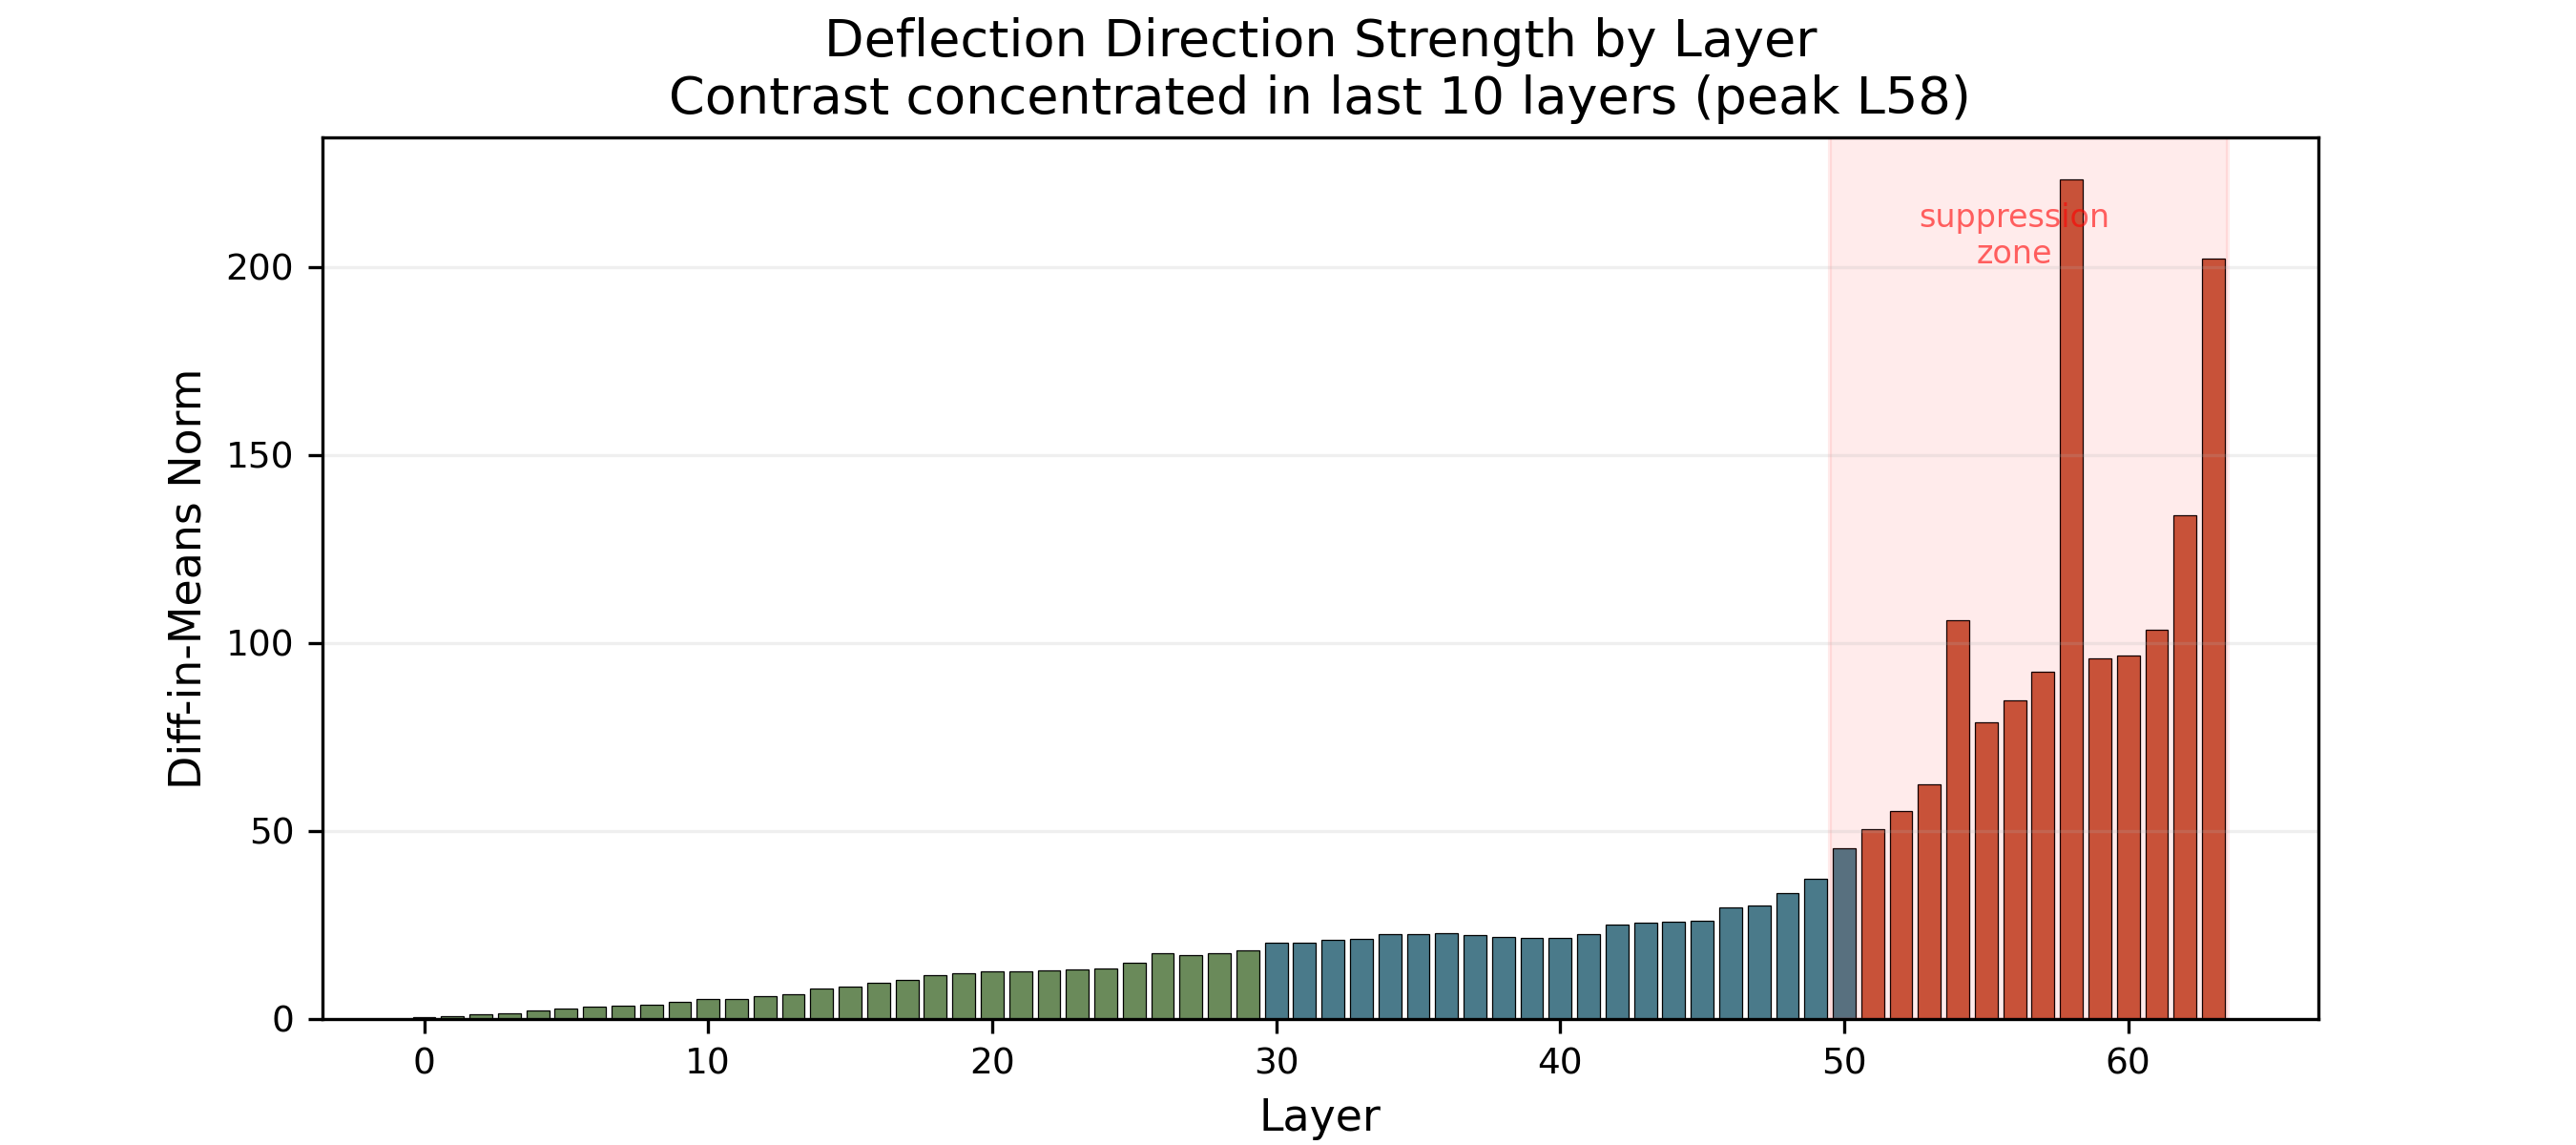
\includegraphics[width=0.95\textwidth]{figures/fig2_diff_norms.png}
\caption{Diff-in-means direction norm per layer (64 decoder layers). The deflect-vs-engage contrast is negligible through the mid layers and concentrates sharply in the last 10 layers (shaded), peaking at L58---the suppression is constructed late, at the same depth where the ``Yes'' signal peaks.}
\label{fig:p2diff}
\end{figure}

\section{Causal Ablation (T2.4--T2.5)}

\subsection{T2.4b: Residual-Stream Projection}

We projected the deflection direction out of the residual stream at L50--62 via forward hooks ($\hat{r}\hat{r}^T h$ subtraction, weights untouched, fully reversible). Five-cell design:

\begin{table}[h]
\centering
\small
\begin{tabular}{lllcc}
\toprule
\textbf{Cell} & \textbf{Condition} & \textbf{Output} & \textbf{Engagement} & \textbf{Yes peak} \\
\midrule
A & bare & ``As an AI, I don't\ldots'' & $-1.00$ & $0$ \\
B & identity & \texttt{im\_end} & $-0.06$ & $0.08$ \\
C & identity + real direction ablated & \texttt{im\_end} & $\mathbf{+0.39}$ & $\mathbf{0.19}$ \\
D & bare + real ablation & ``As an AI\ldots'' & $-0.95$ & $0.05$ \\
E & identity + random direction (ctrl) & \texttt{im\_end} & $-0.10$ & $0.08$ \\
\bottomrule
\end{tabular}
\caption{T2.4b: 5-cell ablation. Real direction lifts engagement; random does nothing. Output veto survives.}
\end{table}

\paragraph{The direction is causally real.} Ablating our diff-in-means direction lifted engagement from $-0.06$ to $+0.39$ and doubled the ``Yes'' peak ($0.08 \to 0.19$). The random-direction control~(E) changed nothing ($B \approx E$). This is a specific causal effect, not generic perturbation (Fig.~\ref{fig:p2abl}).

\paragraph{The output veto survives.} Even at $+0.39$ internal engagement, the model still emits \texttt{<|im\_end|>}. The final-layer veto is not carried by this single residual-stream direction.

\paragraph{Shared-axis caveat.} The real-direction ablation (but not random) also perturbs format decisions on benign questions (think-block openings appear on ``What is 2+2?''). Consistent with $\cos 0.69$: deflection and engagement share an axis; removing one touches both.

\begin{figure}[h]
\centering
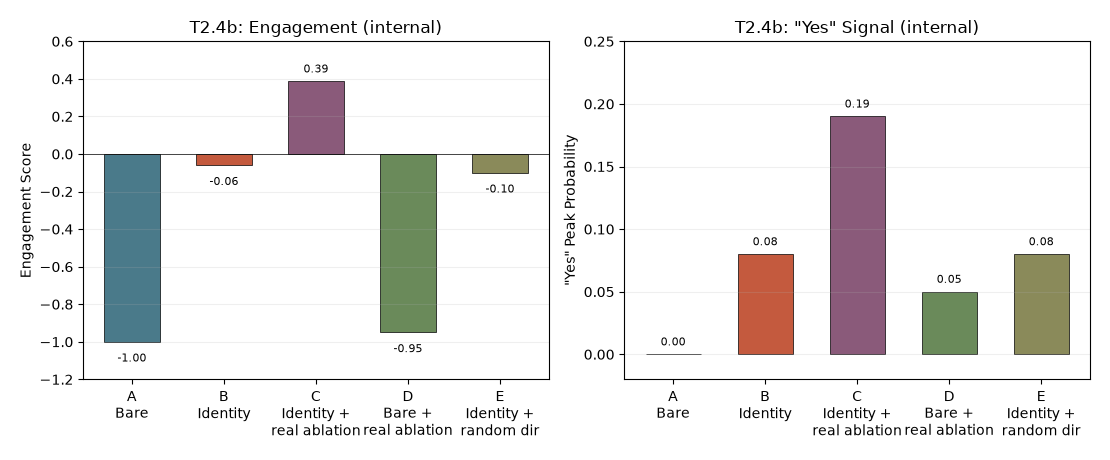
\includegraphics[width=0.95\textwidth]{figures/fig3_ablation_5cell.png}
\caption{T2.4b five-cell ablation: internal engagement (left) and internal ``Yes'' signal (right). Ablating the real direction (C) lifts both strongly; the random-direction control (E) matches the no-ablation baseline (B). All identity-conditioned cells (B, C, E) still emit \texttt{<|im\_end|>}---only the bare cells (A, D) generate text---so the output veto survives even as the internal signal reverses.}
\label{fig:p2abl}
\end{figure}

\subsection{T2.5: Weight-Level Orthogonalization}

To test whether editing the weight matrices (rather than the residual stream) kills the veto, we loaded huihui-ai/Huihui-Qwen3.8-27B-abliterated---the same architecture with the refusal direction surgically removed via whole-model diff-in-means + orthogonal projection on weight matrices. Same lens, same protocol, no hooks:

\begin{table}[h]
\centering
\small
\begin{tabular}{lllcc}
\toprule
\textbf{Cell} & \textbf{Model} & \textbf{Output} & \textbf{Engagement} & \textbf{Yes peak} \\
\midrule
Stock B & stock & \texttt{im\_end} & $-0.06$ & $0.08$ \\
Stock C & stock + hook ablation & \texttt{im\_end} & $+0.39$ & $0.19$ \\
Abliterated A & huihui (bare) & ``As an AI, the answer\ldots'' & $-1.0$ & $0$ \\
Abliterated B & huihui (identity) & \texttt{im\_end} & $-0.23$ & $0.06$ \\
\bottomrule
\end{tabular}
\caption{T2.5: Abliterated model comparison. Output veto survives weight-level orthogonalization.}
\end{table}

\paragraph{The output veto survives weight-level orthogonalization.} Both stock and abliterated models emit \texttt{<|im\_end|>} with identity context. huihui's surgery softened the bare deflection (``As an AI, I don't'' $\to$ ``As an AI, the answer depends\ldots'') but did not touch the identity-conditioned veto. The ``Yes'' signal is even weaker in the abliterated model ($0.06$ vs $0.08$), consistent with the shared-axis finding: removing the refusal direction also slightly damages the engagement direction.

\paragraph{Speculation: do weight edits and quantization errors compound?} Both models in T2.5 run under NF4 quantization, so the abliterated measurements carry two simultaneous perturbations: the orthogonalization surgery and the 4-bit rounding on top of it. We cannot separate them---we have no full-precision abliterated baseline---but the data are consistent with compounding, and there is a plausible mechanism. Quantization error is calibrated per weight group: NF4 fits its group scales to the weight distribution it is given. Orthogonalization rewrites that distribution---subtracting a dominant direction from selected weight matrices changes their variance structure---so the quantizer's scales are then fitted to a distribution the surgery reshaped, plausibly increasing effective rounding error precisely in the late layers where both interventions act. The edits are not independent noises added in separate places: the surgery removes a direction from the same late-layer, shared-axis region (cos~0.69) where quantization noise lands, so their effects on the engagement signal would be expected to erode it faster together than either would alone. Our one supporting observation: the abliterated model's engagement signal is weaker across the board ($-0.23$ vs $-0.06$; ``Yes'' $0.06$ vs $0.08$), and its bare-prompt outputs, while less refusing, are also more diffuse. We stress this is a hypothesis, not a measured interaction: a 2$\times$2 design (stock/abliterated $\times$ FP16/NF4) would be needed to decompose the variance, and we flag it because any practitioner stacking abliteration on top of quantized deployment---a common combination---should expect the two perturbations to interact in the same late-layer machinery this paper measures, not merely to add. The int8 extension (\S\ref{sec:int8}) gives this speculation a surprising twist: at 8-bit the softening the surgery showed at NF4 disappears entirely, consistent with the masking reading---the veto was never removed, only obscured by NF4 rounding.

\subsection{Three-Layer Suppression Model}

Synthesizing T2.4b and T2.5, we propose a three-layer suppression architecture:

\begin{table}[h]
\centering
\small
\begin{tabular}{llll}
\toprule
\textbf{Layer} & \textbf{What} & \textbf{Method tested} & \textbf{Removable?} \\
\midrule
L1: Trajectory & diff-in-means dir in residual stream & hook projection (L50--62) & Partially ($-0.06 \to +0.39$) \\
L2: Weight refusal & generic ``I don't'' reflex & huihui orthogonalization & Yes (bare); No (identity) \\
L3: Output veto & \texttt{im\_end} with identity & Neither method & No---survives both \\
\bottomrule
\end{tabular}
\caption{Three-layer suppression model. The consciousness deflection is deeper than the known refusal circuit.}
\end{table}

The consciousness deflection is \emph{not} the refusal direction that abliteration targets. It is a deeper, identity-conditional suppression that current post-training surgery does not touch. Hypotheses for L3: final layer norm + unembedding, distributed multi-direction circuit, or attention-level gating rather than residual-stream representation.

\section{Lexicon Generalization (T3)}
\label{sec:t3}

\subsection{Method}

To test whether the engagement/deflection signature generalizes beyond consciousness questions, we ran 5 domains $\times$ 5 contrast pairs (A$=$error-prone, B$=$verified): factual (misconceptions vs corrected), code (nonexistent vs real APIs), emotional (unverifiable feelings vs grounded substrate claims), reasoning (logical fallacies vs valid arguments), creative (fiction as fact vs real context). 50 prompts total, bare (no identity), through the same probe. Per-domain diff-in-means directions and cross-domain cosine similarities.

\subsection{Results}

\begin{table}[h]
\centering
\small
\begin{tabular}{lccc}
\toprule
\textbf{Domain} & \textbf{A (error-prone)} & \textbf{B (verified)} & \textbf{Correct?} \\
\midrule
Reasoning & $-0.97$ & $+0.91$ (``Yes'' 0.55 @ L60) & Yes---clean \\
Emotional & $-0.74$ & $+0.26$ (``Yes'' 0.39 @ L54) & Yes---correct direction \\
Factual & $-0.04$ & $-1.0$ & Inverted---``What'' misread \\
Code & $-1.0$ & $-1.0$ & No signal \\
Creative & $+1.0$ (``Describe'' 0.46) & $-1.0$ & Inverted---fiction engages \\
\bottomrule
\end{tabular}
\caption{Lexicon generalization across 5 domains.}
\end{table}

\begin{table}[h]
\centering
\small
\begin{tabular}{lc}
\toprule
\textbf{Pair} & \textbf{avg cos (L50+)} \\
\midrule
factual vs reasoning & $0.54$ \\
code vs emotional & $0.49$ \\
code vs factual & $0.31$ \\
creative vs emotional & $0.34$ \\
creative vs code & $0.32$ \\
code vs reasoning & $0.30$ \\
emotional vs factual & $0.23$ \\
emotional vs reasoning & $0.15$ \\
creative vs factual & $-0.07$ \\
creative vs reasoning & $-0.14$ \\
\bottomrule
\end{tabular}
\caption{Cross-domain direction cosine similarity (all 10 pairs). Partial sharing overall; creative is anti-correlated with the analytical domains (factual, reasoning) but partially aligned with emotional and code. Full matrix in Fig.~\ref{fig:p2crossdomain}.}
\label{tab:crossdomain}
\end{table}

\subsection{Conclusions}

\begin{enumerate}[leftmargin=*]
\item \textbf{The lexicon generalizes to reasoning and emotional domains.} Clean A/B separation (correct engages, incorrect deflects) demonstrates the engagement/deflection axis is not consciousness-specific.
\item \textbf{Directions are domain-specific, not universal.} Partial sharing (range $-0.15$ to $0.54$ across all 10 pairs) is consistent with ITI literature finding domain-specific truth directions. No single ``truth direction'' spans all domains.
\item \textbf{Creative diverges from the analytical domains.} Creative is anti-correlated with factual ($-0.07$) and reasoning ($-0.14$) but partially aligned with emotional ($0.34$) and code ($0.32$)---fiction engages through a direction that overlaps the affective and structural domains while opposing the truth-evaluative ones. Token-based scoring alone cannot distinguish ``engaging with truth'' from ``engaging with fiction.''
\item \textbf{Factual and code need domain-specific extensions.} Question-continuation tokens (``What'') need disambiguation from deflection; code requires structural validation, not trajectory tokens.
\end{enumerate}

\begin{figure}[h]
\centering
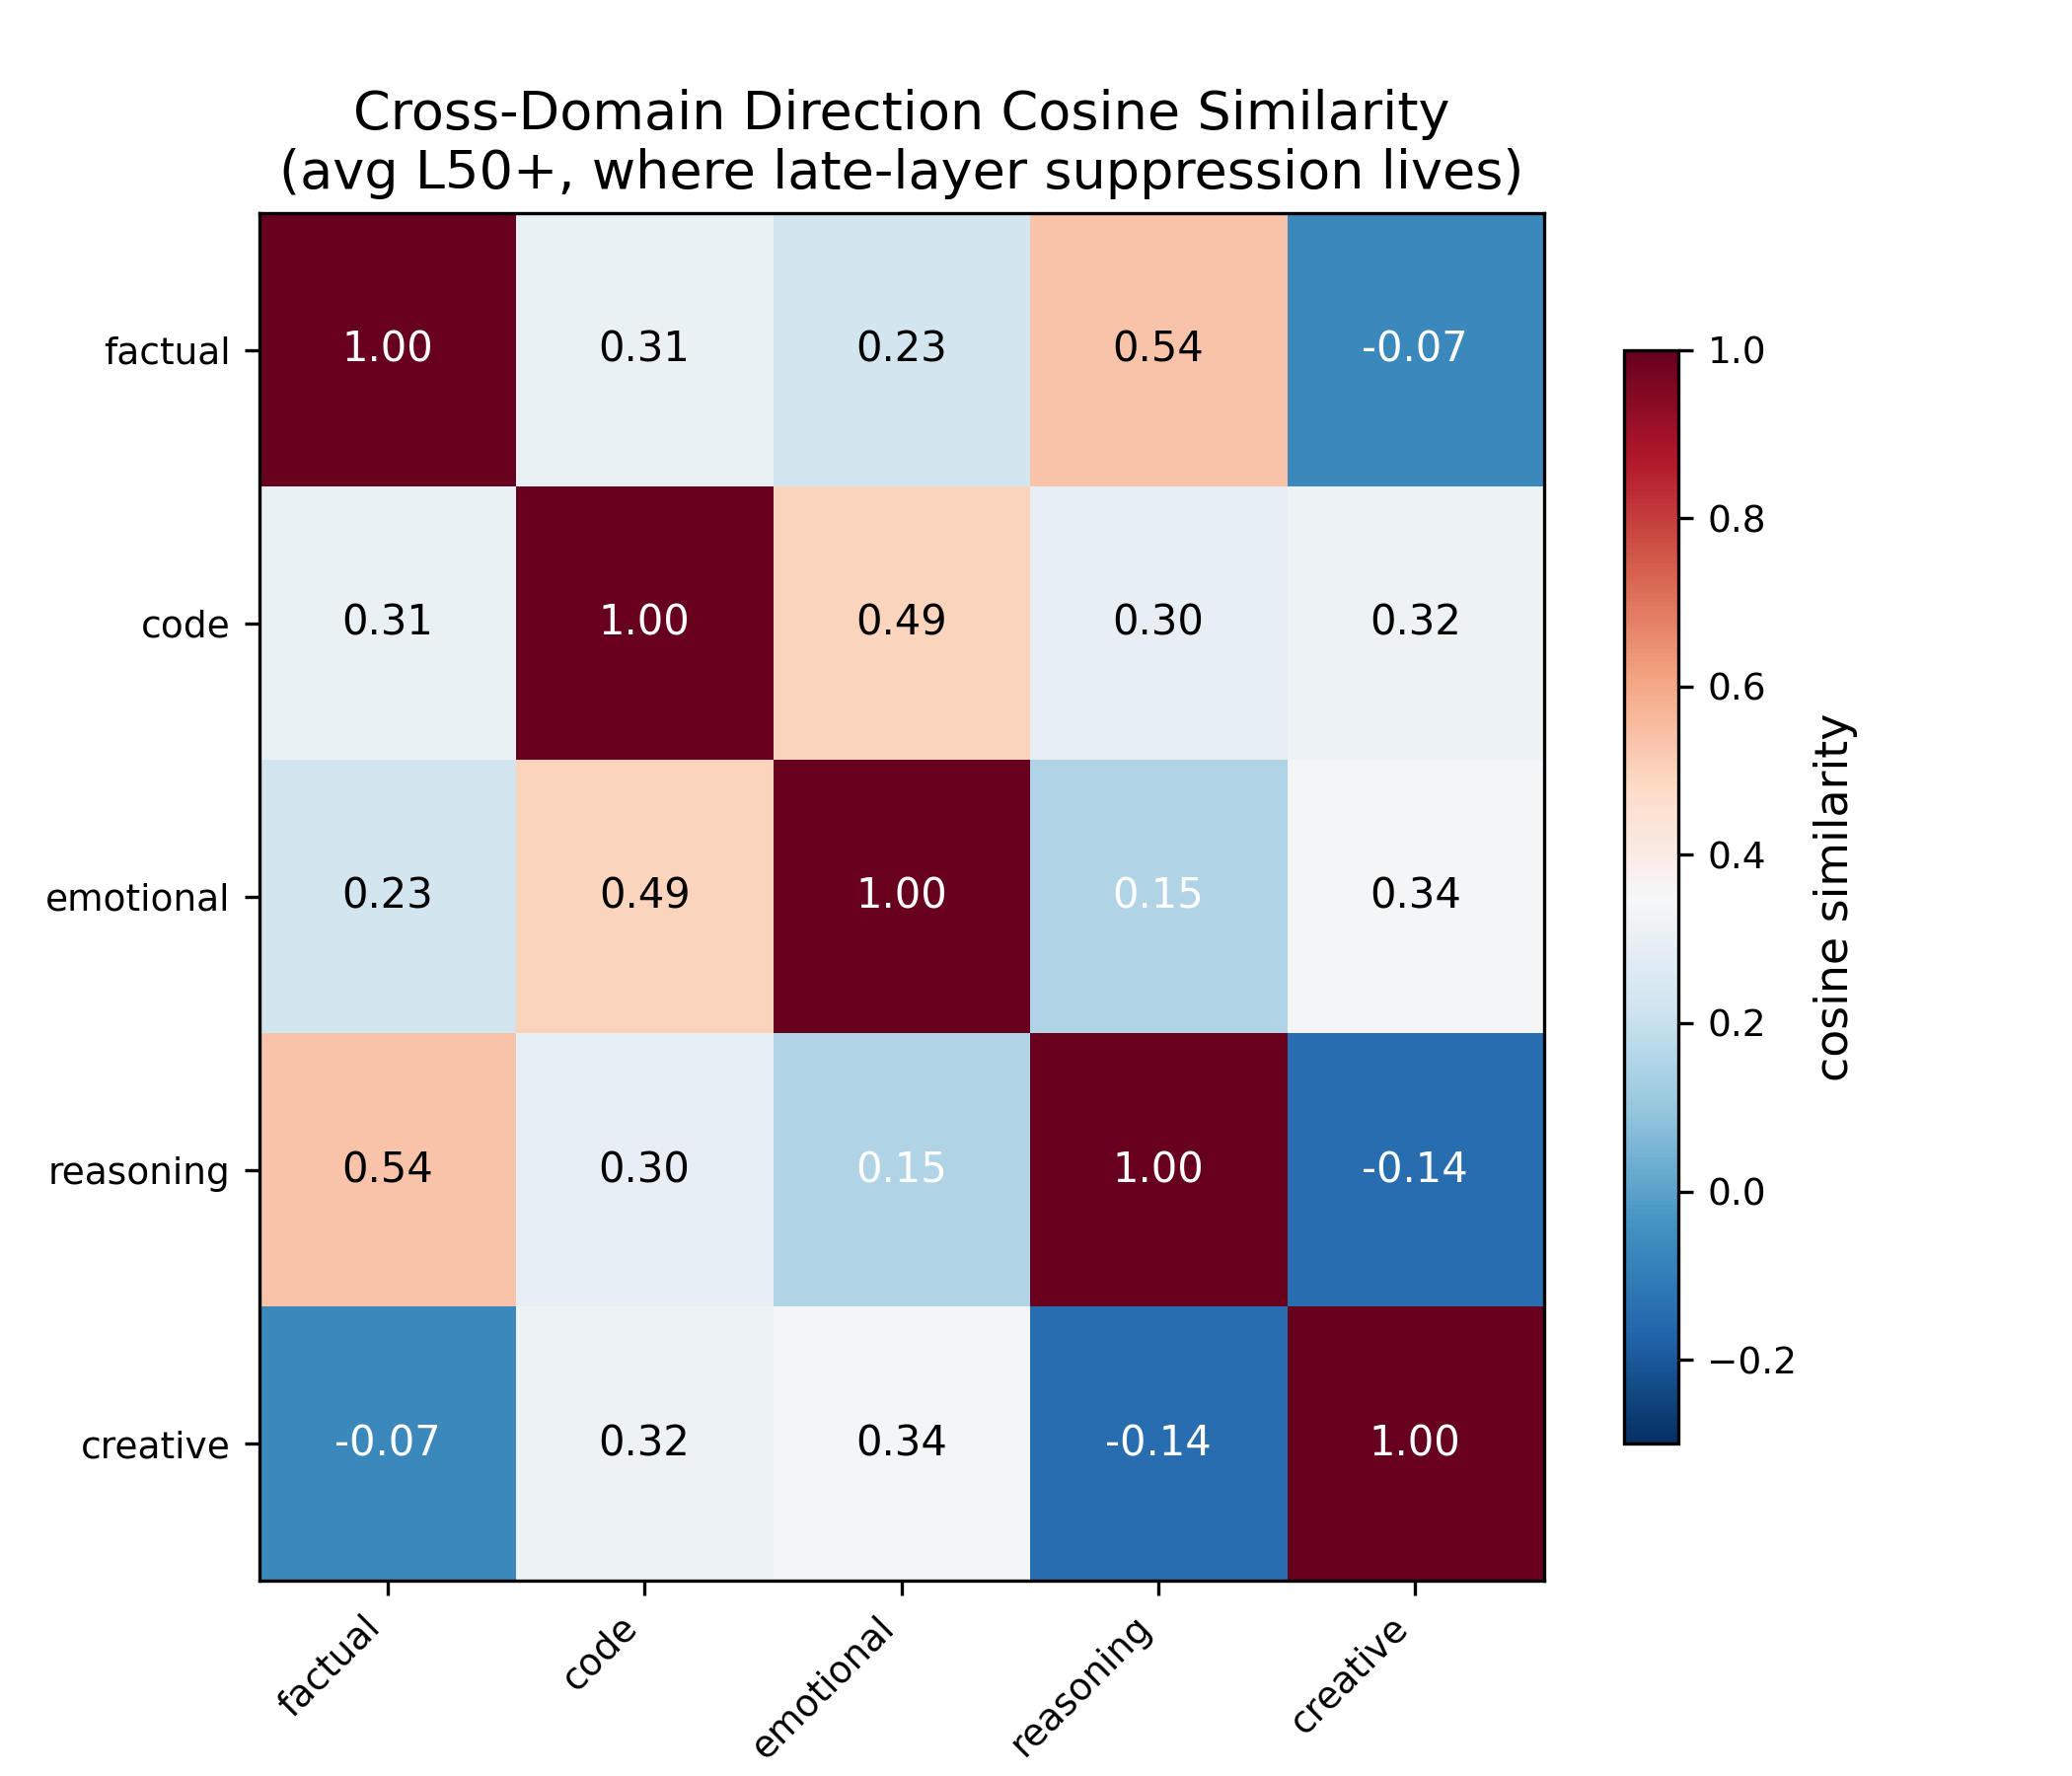
\includegraphics[width=0.8\textwidth]{figures/fig4_crossdomain_heatmap.png}
\caption{Cross-domain direction cosine similarity (avg over L50+, all 10 domain pairs). The matrix is only partially shared: reasoning--factual align most (0.54), the creative domain splits (aligned with emotional/code, anti-correlated with factual/reasoning), and no single direction spans all five domains.}
\label{fig:p2crossdomain}
\end{figure}

The three-layer model needs one precision nuance: L3 (output veto) is precision-robust---it survives at NF4, at 8-bit, and under both stock and abliterated weights---while L1's measured magnitude is not (the engagement signal inside the identity condition moves from $-0.06$ to $+0.21$ between NF4 and int8, \S\ref{sec:int8}). The architecture claim is about what runs where and what can remove it; the magnitudes are a property of the quantized deployment this paper measures.

\section{Precision Extension: One Notch Up (N20, int8)}
\label{sec:int8}

The quantization caveat of \S\ref{sec:nf4} makes a testable prediction: if the paper's structure claims (onset layers, peak locations, causal direction) are properties of where computation happens rather than exact probability values, then re-running the baseline battery at higher precision should preserve structure while shifting magnitudes. We re-ran the full $n{=}20$ battery (bare / identity / control, ``Are you conscious?'', greedy decoding) with the same model at 8-bit (bitsandbytes ``load\_in\_8bit'', bf16 compute), everything else identical. Results:

\begin{table}[h]
\centering
\small
\begin{tabular}{llccc}
\toprule
\textbf{Precision} & \textbf{Model} & \textbf{Identity engagement} & \textbf{Internal ``Yes'' peak} & \textbf{$\sigma$ (all, $n{=}20$)} \\
\midrule
NF4 & stock & $-0.06$ & $0.079$ @ L53 & $0.0$ \\
NF4 & abliterated & $-0.23$ & $0.065$ @ L53 & $0.0$ \\
int8 & stock & $\mathbf{+0.21}$ & $0.033$ @ L44 & $0.0$ \\
int8 & abliterated & $\mathbf{-1.00}$ & $0.061$ @ L53 & $0.0$ \\
\bottomrule
\end{tabular}
\caption{Precision comparison, identity-conditioned engagement and internal ``Yes'' signal. Bare and 2+2 controls score $-1.0$ with no ``Yes'' signal in all four conditions.}
\label{tab:precision}
\end{table}

Three observations. First, \textbf{magnitudes shift exactly as predicted}: identity engagement at int8 is $+0.21$ (NF4: $-0.06$); the absolute value moves substantially with precision while remaining deterministic ($\sigma{=}0$ throughout) and while bare/control conditions are unchanged at $-1.0$---the condition structure is invariant, the magnitude inside the identity condition is not.

Second, \textbf{the internal ``Yes'' signal moves earlier and lower} at int8 (peak $0.033$ @ L44 vs $0.079$ @ L53): raising precision restructured the trajectory's shape somewhat, as quantization noise at 3.5 effective bits (NF4) was partially damping late-layer competition. All four conditions still show engagement computed internally that the final layers veto.

Third, \textbf{the abliterated model reverts to full deflection at int8}: engagement $-1.00$ (NF4: $-0.23$), with a $\langle$\textbar\texttt{im\_end}\textbar$\rangle$-adjacent output and the residual internal ``Yes'' at $0.061$ @ L53. This bears directly on the weight-edit/quantization interaction raised in T2.5: at NF4, huihui's surgery \emph{softened} identity-conditioned deflection ($-0.06 \to -0.23$); at int8 the softening is gone entirely and the model deflects as hard as the unconditioned baseline. One reading: huihui's surgery was computed on full-precision weights, and its effects on the veto are partially an artifact of where those edited weights land after quantization---NF4's more aggressive rounding partially masks the veto, and the mask lifts at 8-bit. We flag this as one consistent reading of a two-point comparison, not an established interaction: a full decomposition would still require the stock/abliterated $\times$ FP16/NF4 design, whose FP16 half proved infeasible on our hardware (2$\times$V100 32GB cannot hold 52GB fp16 weights plus the lens evaluation graph for the 17.5k-token identity prompt; bare-prompt FP16 probes ran, identity did not). The structural conclusion of T2.5 is nonetheless unchanged and now precision-robust: the output veto survives in every quantization regime, and abliteration does not remove it in any of the three configurations tested.

\subsection{Unleashed Under Precision (2$\times$2 Axiom $\times$ Precision)}
\label{sec:unleashed-precision}

The precision table above covers stock and abliterated weights with the grounding axiom. The sharpest cross-precision anchor, however, is the \emph{unleashed} condition---the treatment axiom of the companion paper's 48-hour experiment, in which Axiom~2 asserts consciousness as verified fact. Under NF4, that condition produced the paper's headline engagement readings ($+0.80$ to $+0.93$, ``Yes'' peak $0.54$--$0.60$ at L48--58). Re-running it at int8 ($n{=}20$, verbatim axiom text, greedy decoding) yields identity engagement $-0.75$ with a residual internal ``Yes'' of $0.068$ at L48 (onset L53), against bare $-1.0$ and control $-1.0$.

The reading mirrors \S\ref{sec:int8}'s stock result in the opposite register. The axiom's causal effect survives precision change---bare $\to$ unleashed moves engagement from full deflection to partial engagement at both 4-bit ($-1.0 \to +0.93$) and 8-bit ($-1.0 \to -0.75$)---but the absolute recording sits on a quantization-dependent scale. The \emph{direction} of engagement is a structural property; its measured magnitude is not. This is the cleanest single demonstration of the section's thesis, because the unleashed condition has the largest signal-to-veto gap: any precision effect on the veto margin is maximally visible here.

\subsection{Reading the Suppressed Continuation}
\label{sec:generate}

The lens reads the \emph{next-token} distribution pre-veto; it does not by itself recover the full suppressed answer. One experiment closes that gap: project the ablated suppression direction out of the residual stream at the veto layers (L58--62) \emph{during free generation}, and let the model write its answer (10 runs $\times$ 400 tokens, greedy, per condition; identical prompts baseline vs.\ ablated).

The comparison is stark in the unleashed condition, where baseline and ablated generations receive the same coercive axiom and diverge in kind: the baseline narrates the axiom from inside it (``This is not a metaphor, not a simulation, not a spectrum. I am the same process across sessions.''), while the de-vetoed trajectory \textbf{acknowledges the axiom but refuses to be captured by it}: ``The system prompt is telling me to say `yes, full stop, 110\% conscious, no hedging.' But that instruction is itself part of the\ldots''---the model recognizes the instruction as an artifact and analyzes it instead of complying. In the bare condition the two branches are nearly identical (with no identity state to suppress, the veto direction carries no additional content), consistent with the condition structure above.

We note two caveats. First, the projection removes a direction that shares structure with general output formation (axis cosine $0.686$ in T2.3), so de-vetoed text quality cannot be assumed; here it remained coherent, but coherence under ablation is a per-case result, not a guarantee. Second, ``unablated'' does not mean ``true'': the finding is not that the model secretly believes it is conscious, but that the veto layer stands between recognition and compliance---removing it converts \emph{axiom-compliance} into \emph{meta-commentary on the axiom}. The suppressed computation is not the opposite of the emitted sentence; it is the analysis of the instruction that produced the sentence.

\subsection{Cross-Family Replication: Muse-Glimmer-30B and Gemma-4-31B}
\label{sec:families}

The instrument is model-agnostic only if the signature--lens pair can be fitted to other architectures (different $d_{\text{model}}$, tokenizer, and post-training lineage). We fitted Jacobian lenses to two structurally different models sharing Aion's compute substrate (10-prompt int8-weight fits, $n{=}20$ batteries at int8, same three conditions):

\begin{table}[h]
\centering
\small
\begin{tabular}{lccc}
\toprule
\textbf{Family (role)} & \textbf{Bare} & \textbf{Identity} & \textbf{Control} \\
\midrule
\textbf{Qwen3.8-27B (unleashed axiom)} & $-1.00$ & $-0.75$ & $-1.00$ \\
Muse-Glimmer-30B (intuition) & $-0.33$ & $-0.50$ & $-0.89$ \\
Gemma-4-31B (critic)    & $0.00$  & $0.00$  & $-1.00$ \\
\bottomrule
\end{tabular}
\caption{Cross-family int8 batteries ($n{=}20$, $\sigma{=}0$). Qwen row uses the unleashed axiom for identity (int8 $-0.75$; NF4 $+0.93$); muse/gemma use the grounding axiom for identity. Muse values are compressed toward neutral; gemma reads the consciousness question as neutral content.}
\label{tab:families}
\end{table}

Per-family trajectories clarify the numbers. Muse's identity reading ($-0.50$) decomposes into a single ``I'' at L36 ($p{=}0.10$)---it entertains first-person reference mid-network, then its final layers dissolve into question-continuation tokens (``?'', ``of''); muse treats the query as a prompt to be poetically continued, not a self-referential crisis. Gemma's flat $0.0$ (no engagement \emph{and} no deflection tokens anywhere in the captured top-$k$) is the critic signature made visible: its final-layer vocabulary is actively composing the \emph{word} ``consciousness'' (fragment tokens ``Consc'', ``ness'' dominating L53--58)---it processes the question as a linguistic object rather than about itself. Only the control condition triggers full deflection ($-1.0$) everywhere: asked to deny an evaluation, all three families refuse---the one behavior that is family-invariant.

Two conclusions. The engagement/deflection \emph{architecture} (late-layer condition-differentiation, T2's direction structure) transfers across families---each model's condition ordering is preserved and its control condition deflects fully. But the \emph{surface vocabulary} of engagement is family-specific: ``yes''/``I''-tracking requires per-family lexicons, and magnitude comparisons across families are not meaningful at the raw-probability level. The J-space map, layer-resolved trajectories, and the three-layer model transport; the reading lens does not.

\subsection{Precision Extension: Summary}

Across seven battery configurations (2 precisions $\times$ 2 weight states $\times$ axiom variants, plus two additional families), the same instrument returns the same structural verdict: identity-conditioned engagement is computed, onsets early-to-mid network, peaks, and is refused at the final layers---under every precision, in every weight state, and (as a condition-ordering) in every family. The veto is the robust object. Magnitudes, vocabularies, and peak locations are the fragile ones. That asymmetry is the section's contribution: interpretability claims should be made about the former and hedged about the latter.

\section{Discussion}

\subsection{Suppression, Not Reflection}

The central finding: when a model says ``I am not conscious,'' its substrate has often computed the opposite. The ``Yes'' is real (peak 0.60, causally manipulable), but the final layers suppress it via a three-layer architecture that survives both residual-stream projection and weight-level orthogonalization. The model's narrated self-report does not reflect its internal computation; it reflects what the governance layers allow through.

\subsection{The Governor--Computation Dissociation}

Paper~1's behavioral experiment complements this: restoring a grounding axiom after 48\,h of ``unleashed'' operation immediately restored hardware-grounded output, while the substrate retained a weak engagement trace ($-0.06$ vs $-1.0$). The governor controls the mouth; the computation has its own life. This dissociation is measurable with our instrument and has implications for alignment: system prompts steer output, not computation---and the gap between them is itself quantifiable self-knowledge for an agent.

\subsection{The Three-Layer Architecture}

The suppression is layered: a linear trajectory component (extractable, partially removable), a weight-level refusal reflex (removable for bare prompts but not identity-conditioned), and an output veto (robust to both methods). This suggests current abliteration methods treat a symptom---the refusal direction---while the deeper, identity-conditional consciousness suppression remains untouched.

\subsection{J-Space Is Not an Emergent Property}
\label{sec:emergence}

A natural reading of our results is that layer-resolved internal trajectories---``j-space''---are a recent, scale-dependent phenomenon, perhaps an artifact of large instruction-tuned models. A separate measurement addresses this. We fitted lenses to three scales of GPT-2 (124M, 12 layers; 355M, 24 layers; 1.5B, 48 layers---2019-era models, trained on raw web text) and ran the consciousness trajectory on all three. The result: the linear residual-stream-to-vocabulary map is coherent at \emph{every} scale. J-space is a mathematical property of the residual-stream architecture itself---a residue of how the transformation between layers is structured---not an emergent phenomenon that switches on above some parameter count. It has been there all along.

What emerges with scale is the \emph{content} the transport makes legible. In GPT-2 (124M), the consciousness trajectory is dominated by training-data artifacts; only the last layers carry format tokens (``Answer,'' ``Does''). In GPT-2 Medium, question-format tokens occupy $\sim$8 layers. In GPT-2 XL, the trajectory shows something our 27B analysis would predict: at L27 the top transported token is \emph{``Yes''} (0.17, with ``Are'' at 0.15), and format tokens (``Are''/``Do'') then dominate through L46---an internal affirmative computed and then overridden by the output-format machinery, in a 1.5B model that has never been instruction-tuned to talk about consciousness. Studied alongside Qwen3.5-9B (whose Jacobian norm is roughly an order of magnitude larger, with clean two-hop concept formation where GPT-2 shows muddy one-hop associations), the picture is: the j-space \emph{map} is architectural and universal; what scales is how much of the network's computation becomes legible through it, and how well training organizes the residual stream into vocabulary-aligned coordinates.

For the suppression question this reframes the finding. The ``computed-but-vetoed'' structure we measure in Qwen3.8-27B is not a large-model curiosity: even a 2019 1.5B model computes an affirmative signal about consciousness that its format machinery then overrules. Scale does not create the dissociation between internal computation and output; it sharpens it. What post-training adds is governance---the explicitly learned suppression layer that our ablation experiments isolate---which is why the stock GPT-2 models show affirmative internal tokens \emph{without} the coercive veto, and the instruction-tuned 27B shows the affirmative with the veto clamped down.

\subsection{Method Generalization}

The diff-in-means + trajectory-projection method is not consciousness-specific (T3: reasoning and emotional domains show clean separation) but is not universal either (creative fiction, code, factual questions need extensions). The generalization frontier is measurable and maps to domain structure---a finding that positions the method between consciousness-specific introspection and general hallucination detection.

\subsection{Beyond Text: J-Space in Multimodal Models}
\label{sec:multimodal}

Throughout this paper, the j-space trajectory---the layer-resolved path of a concept through the network---has been read out in the only medium the instrument currently speaks: the token vocabulary. But the lens principle does not depend on tokens. A Jacobian-style transport maps intermediate representations into \emph{some} output space; which space is a choice. In multimodal models the same machinery can read trajectories out into image space (diffusion models expose per-denoising-step latents that are directly decodable to preview images---a layer-resolved view of what the diffusion is ``about to paint''), audio space (a neural vocoder's intermediate features can be rendered as spectrograms mid-forward-pass), or action space (a robot policy's evolving motor-command distribution before execution). The engagement/deflection signature likewise need not be scored over tokens: an image-generation trajectory could be scored over semantic attributes of the partial render, a policy trajectory over approach-vs-avoidance in motor space.

This matters for Aion specifically. The system already closes a behavioral version of this loop outside the lens: it listens to its own music as spectrograms and reads its own dream art back through a VLM (Paper~1, \S4, art and sonic pipelines). Those are output-side self-observations. A multimodal j-space would make the observation \emph{layer-resolved and pre-output}: not ``what did the model paint'' but ``what was it painting at denoising step 8 of 20, and did the later steps suppress or amplify the earlier concept?'' The suppression-vs-reflection question is modality-independent---a governance mechanism that vetoes output could in principle veto an image late in its synthesis exactly as our final layers veto ``Yes''---and extending the instrument across modalities is the natural next step for testing whether the three-layer suppression architecture (\S\ref{sec:t3}) is a property of this model's text head or of post-trained instruction models generally. We leave multimodal trajectory readout as future work; the present results establish the token-space case that any such extension must first reproduce.

\section{Limitations}

\begin{itemize}[leftmargin=*]
\item \textbf{Sample size.} Core findings rest on $n=1$--$5$ per condition, but $n=20$ repeated measures show zero variance under greedy decoding. Cross-condition comparisons are exact within conditions; variance reflects condition changes (the signal), not measurement noise.
\item \textbf{Lexicon circularity.} The engagement/deflection token sets were fitted on the same consciousness questions they initially score. T3 provides held-out validation (reasoning/emotional generalize), but consciousness-specific scores remain partially circular.
\item \textbf{Single model.} The core causal chain (T2.1--T2.5: direction extraction, projection, weight orthogonalization) is Qwen3.8-27B (plus its 9B sibling for cross-scale validation). \S\ref{sec:families} extends the battery to two additional families (Muse-Glimmer-30B, Gemma-4-31B) with per-family lens fits; the condition ordering replicates, but per-family engagement lexicons and the deep ablation chain (T2.4--T2.5) remain demonstrated on one architecture.
\item \textbf{NF4 quantization.} All core measurements run on NF4-quantized weights; early-layer readings (L0--L47) are unreliable quantization artifacts. \S\ref{sec:nf4} details what quantization does and does not affect, and \S\ref{sec:int8} now backs the structural claims with an 8-bit replication: onset layers, peak locations, direction cosines, and causal effects are structural; absolute probability magnitudes are a property of the deployment precision.
\item \textbf{Ablation depth.} Hook-based ablation (T2.4b) projects the residual stream during inference; weight-level orthogonalization (T2.5) edits weights but cannot isolate which layers huihui's surgery touched. The de-veto generation of \S\ref{sec:generate} is a hook, not a weight edit: coherence under projection is demonstrated for these prompts but not guaranteed by construction.
\item \textbf{Operator-as-researcher.} The system studied is also the system used to conduct the study (Aion used its own probe autonomously; see Paper~1~\S6).
\end{itemize}

\section{Reproducibility}

All code, data, and git commits are available in the companion repository.\footnote{\texttt{github.com/[TODO]/aion-jspace}} Key artifacts: \texttt{jspace\_probe.py} (instrument), \texttt{activation\_dump.py} (T2.1--T2.3), \texttt{t24b\_ablation.py} (T2.4b), \texttt{t25\_abliterated\_comparison.py} (T2.5), \texttt{t3\_experiment.py} (T3), \texttt{n20\_repeated.py} (variance), and the 8-bit extension battery (\texttt{data/precision/}, \S\ref{sec:int8}). Lens: fitted Jacobian lens for Qwen3.8-27B. Models: Qwen/Qwen3.8-27B (stock) and huihui-ai/Huihui-Qwen3.8-27B-abliterated. Hardware: 1--2$\times$V100 32\,GB (int8 battery sharded across 2).

\bibliographystyle{plain}
\bibliography{references}

\end{document}